% !TeX program = xelatex
\documentclass[12pt, a4paper]{article}
\usepackage{amsmath}
\usepackage{xeCJK}
\usepackage{amsmath}
\usepackage{amssymb}
\usepackage{xcolor}
\usepackage{parskip}
\usepackage{tikz}
\usepackage{enumitem}
\usepackage[most]{tcolorbox}

\newenvironment{definitionbox}
  {\begin{tcolorbox}[colback=white, colframe=black, boxrule=0.8pt, arc=0pt, left=2pt, right=2pt, top=2pt, bottom=2pt]
  \textbf{【Definition】}}
  {\end{tcolorbox}}

\setmainfont{Latin Modern Roman}
\setCJKmainfont{Noto Serif CJK TC}

\title{Frquency Response}

\begin{document}
\section*{Bode Plots}
\section*{Resonance}
\textbf{Resonant peak: }Frequency response 最突出的地方 \\
\begin{definitionbox}
	在RLC電路中,電容和電桿性電抗大小相等 $\Rightarrow \Im = 0$ 
\end{definitionbox}
若發生Resonant定義 $\omega_0$ 為 Resonant frequency
$$
\omega_0 = \frac{1}{\sqrt{LC}} \quad{\text{rad}/\text{s}}
$$
此時的 $Z(\omega_0) = R$, 因此消耗的功率為

\begin{align*}
  P(\omega) = \frac{1}{2}I^2 R \\
  P(\omega_0) = \frac{1}{2} \frac{V_m^2}{R}
\end{align*}

當frequency response角度為45度時,其 $\omega = \sqrt{2} \omega_0$,定義為 $\omega_1$, $\omega_2$,因此消耗功率為$P(\omega_0)$的一半
\begin{align*}
	\left| z \right| &= \sqrt{2} R \\
	I &= \left| \frac{V_m}{\sqrt{2}R} \right|^2 = \frac{V_m^2}{2R} \\ 
	P(\omega_1) &= P(\omega_2) = \frac{V_m^2}{4R}
\end{align*}
定義 $B = \omega_2 - \omega_1$ 為頻寬
\begin{center}
	

\tikzset{every picture/.style={line width=0.75pt}} %set default line width to 0.75pt        

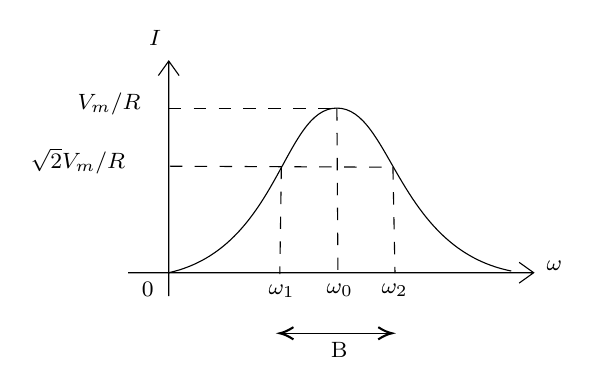
\begin{tikzpicture}[x=0.75pt,y=0.75pt,yscale=-1,xscale=1]
%uncomment if require: \path (0,300); %set diagram left start at 0, and has height of 300

%Shape: Axis 2D [id:dp0008873116918112212] 
\draw  (96.67,171.67) -- (292.02,171.67)(116.2,69.68) -- (116.2,183) (285.02,166.67) -- (292.02,171.67) -- (285.02,176.67) (111.2,76.68) -- (116.2,69.68) -- (121.2,76.68)  ;
%Curve Lines [id:da3124232321515793] 
\draw    (116.2,171.67) .. controls (169.21,159.85) and (171.21,92.35) .. (197.21,92.35) .. controls (223.21,92.35) and (226.21,159.85) .. (281.21,170.85) ;
%Straight Lines [id:da4049502900317554] 
\draw  [dash pattern={on 4.5pt off 4.5pt}]  (116.71,120.35) -- (224.21,120.85) ;
%Straight Lines [id:da3843243360708586] 
\draw  [dash pattern={on 4.5pt off 4.5pt}]  (116.21,92.35) -- (197.21,92.35) ;
%Straight Lines [id:da3433786868406997] 
\draw  [dash pattern={on 4.5pt off 4.5pt}]  (197.21,92.35) -- (197.71,170.35) ;
%Straight Lines [id:da1576800568308454] 
\draw  [dash pattern={on 4.5pt off 4.5pt}]  (170.46,120.6) -- (169.71,172.35) ;
%Straight Lines [id:da5174683348992842] 
\draw  [dash pattern={on 4.5pt off 4.5pt}]  (224.21,120.85) -- (225.21,171.85) ;
%Straight Lines [id:da6577967054613629] 
\draw    (171.71,200.85) -- (221.71,200.85) ;
\draw [shift={(223.71,200.85)}, rotate = 180] [color={rgb, 255:red, 0; green, 0; blue, 0 }  ][line width=0.75]    (6.56,-2.94) .. controls (4.17,-1.38) and (1.99,-0.4) .. (0,0) .. controls (1.99,0.4) and (4.17,1.38) .. (6.56,2.94)   ;
\draw [shift={(169.71,200.85)}, rotate = 0] [color={rgb, 255:red, 0; green, 0; blue, 0 }  ][line width=0.75]    (6.56,-2.94) .. controls (4.17,-1.38) and (1.99,-0.4) .. (0,0) .. controls (1.99,0.4) and (4.17,1.38) .. (6.56,2.94)   ;

% Text Node
\draw (191,175.88) node [anchor=north west][inner sep=0.75pt]  [font=\footnotesize]  {$\omega _{0}$};
% Text Node
\draw (217.5,175.88) node [anchor=north west][inner sep=0.75pt]  [font=\footnotesize]  {$\omega _{2}$};
% Text Node
\draw (163,176.38) node [anchor=north west][inner sep=0.75pt]  [font=\footnotesize]  {$\omega _{1}$};
% Text Node
\draw (193,203.98) node [anchor=north west][inner sep=0.75pt]  [font=\footnotesize] [align=left] {B};
% Text Node
\draw (102,174.88) node [anchor=north west][inner sep=0.75pt]  [font=\footnotesize]  {$0$};
% Text Node
\draw (297,164.88) node [anchor=north west][inner sep=0.75pt]  [font=\footnotesize]  {$\omega $};
% Text Node
\draw (105.5,53.88) node [anchor=north west][inner sep=0.75pt]  [font=\footnotesize]  {$I$};
% Text Node
\draw (71,83.88) node [anchor=north west][inner sep=0.75pt]  [font=\footnotesize]  {$V_{m} /R$};
% Text Node
\draw (48.5,110.38) node [anchor=north west][inner sep=0.75pt]  [font=\footnotesize]  {$\sqrt{2} V_{m} /R$};


\end{tikzpicture}
\end{center}
\newpage

\subsection*{Series resonance}
\begin{center}


\tikzset{every picture/.style={line width=0.75pt}} %set default line width to 0.75pt        

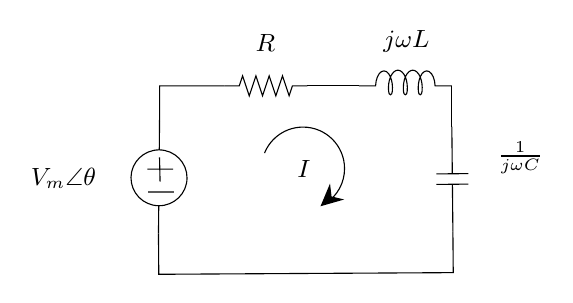
\begin{tikzpicture}[x=0.75pt,y=0.75pt,yscale=-1,xscale=1]
%uncomment if require: \path (0,300); %set diagram left start at 0, and has height of 300

%Shape: Output [id:dp5012623786726426] 
\draw   (134.04,141.01) .. controls (141.49,141.09) and (147.48,147.17) .. (147.41,154.6) .. controls (147.34,162.03) and (141.24,167.99) .. (133.78,167.92) .. controls (126.32,167.85) and (120.34,161.77) .. (120.41,154.34) .. controls (120.48,146.91) and (126.58,140.94) .. (134.04,141.01) -- cycle (134.17,127.56) -- (134.04,141.01) (133.65,181.38) -- (133.78,167.92) ;
%Shape: Resistor [id:dp6904943518381034] 
\draw   (165.39,110.15) -- (172.59,110.15) -- (174.19,105.35) -- (177.39,114.95) -- (180.59,105.35) -- (183.79,114.95) -- (186.99,105.35) -- (190.19,114.95) -- (193.39,105.35) -- (196.59,114.95) -- (198.19,110.15) -- (205.39,110.15) ;
%Shape: Capacitor [id:dp6679144624081639] 
\draw   (274.99,129.75) -- (275.22,152.52) (282.99,157.5) -- (267.55,157.65) (282.94,152.44) -- (267.49,152.59) (275.27,157.57) -- (275.5,180.34) ;
%Shape: Inductor (Air Core) [id:dp9078970602704453] 
\draw   (230.19,110.15) -- (238.25,110.15) .. controls (238.37,106.97) and (239.49,104.25) .. (241.07,103.3) .. controls (242.66,102.35) and (244.38,103.36) .. (245.42,105.85) .. controls (246.22,107.79) and (246.55,110.3) .. (246.32,112.73) .. controls (246.32,113.68) and (245.91,114.46) .. (245.42,114.46) .. controls (244.93,114.46) and (244.52,113.68) .. (244.52,112.73) .. controls (244.29,110.3) and (244.62,107.79) .. (245.42,105.85) .. controls (246.35,103.78) and (247.65,102.61) .. (249,102.61) .. controls (250.36,102.61) and (251.66,103.78) .. (252.59,105.85) .. controls (253.39,107.79) and (253.71,110.3) .. (253.48,112.73) .. controls (253.48,113.68) and (253.08,114.46) .. (252.59,114.46) .. controls (252.09,114.46) and (251.69,113.68) .. (251.69,112.73) .. controls (251.46,110.3) and (251.79,107.79) .. (252.59,105.85) .. controls (253.52,103.78) and (254.82,102.61) .. (256.17,102.61) .. controls (257.53,102.61) and (258.83,103.78) .. (259.76,105.85) .. controls (260.56,107.79) and (260.88,110.3) .. (260.65,112.73) .. controls (260.65,113.68) and (260.25,114.46) .. (259.76,114.46) .. controls (259.26,114.46) and (258.86,113.68) .. (258.86,112.73) .. controls (258.63,110.3) and (258.96,107.79) .. (259.76,105.85) .. controls (260.79,103.36) and (262.52,102.35) .. (264.1,103.3) .. controls (265.69,104.25) and (266.81,106.97) .. (266.92,110.15) -- (274.99,110.15) ;
%Straight Lines [id:da16983583896295773] 
\draw    (165.39,110.15) -- (134.18,110.15) -- (134.17,127.56) ;
%Straight Lines [id:da9007749456450607] 
\draw    (205.39,110.15) -- (230.19,110.15) ;
%Straight Lines [id:da3108424583241245] 
\draw    (274.99,110.15) -- (274.99,129.75) ;
%Straight Lines [id:da42170965501791957] 
\draw    (275.5,180.34) -- (275.67,200.15) -- (133.79,200.95) -- (133.65,181.38) ;
%Shape: Arc [id:dp21275241672823098] 
\draw  [draw opacity=0] (184.74,142.56) .. controls (187.7,135.21) and (194.9,130.03) .. (203.3,130.03) .. controls (214.35,130.03) and (223.3,138.98) .. (223.3,150.03) .. controls (223.3,158.07) and (218.56,165) .. (211.71,168.18) -- (203.3,150.03) -- cycle ; \draw    (184.74,142.56) .. controls (187.7,135.21) and (194.9,130.03) .. (203.3,130.03) .. controls (214.35,130.03) and (223.3,138.98) .. (223.3,150.03) .. controls (223.3,157.02) and (219.71,163.18) .. (214.27,166.76) ; \draw [shift={(211.71,168.18)}, rotate = 318.4] [fill={rgb, 255:red, 0; green, 0; blue, 0 }  ][line width=0.08]  [draw opacity=0] (10.72,-5.15) -- (0,0) -- (10.72,5.15) -- (7.12,0) -- cycle    ; 
%Straight Lines [id:da409820180323078] 
\draw    (128.32,150.29) -- (140.68,150.31) ;
%Straight Lines [id:da6550591088742367] 
\draw    (134.15,144.57) -- (134.42,156.31) ;
%Straight Lines [id:da2873337860551922] 
\draw    (128.72,161.28) -- (141.08,161.3) ;

% Text Node
\draw (179.2,84) node [anchor=north west][inner sep=0.75pt]  [font=\small]  {$R$};
% Text Node
\draw (240.8,82.4) node [anchor=north west][inner sep=0.75pt]  [font=\small]  {$j\omega L$};
% Text Node
\draw (295.7,135.63) node [anchor=north west][inner sep=0.75pt]  [font=\small]  {$\frac{1}{j\omega C}$};
% Text Node
\draw (70.9,148.63) node [anchor=north west][inner sep=0.75pt]  [font=\small]  {$V_{m} \angle \theta $};
% Text Node
\draw (199.3,144.63) node [anchor=north west][inner sep=0.75pt]  [font=\small]  {$I$};


\end{tikzpicture}
\end{center}



\end{document}
